\subsection{Алгоритм для языка Дика на одном типе скобок}

{\bf Алгоритм из статьи}~\cite{Mathiasen21}

\begin{definition}[Bell-shaped путь]
    Путь, который понимается строго вверх, потом сколько-то идёт ровно ($\eps$-рёбра), потом спускается строго вниз
\end{definition}

Ищем bell-shaped пути: удваиваем рёбра, ищем пути с серединкой из bell-shaped пути поменьше (так $\log n^2$ раз).

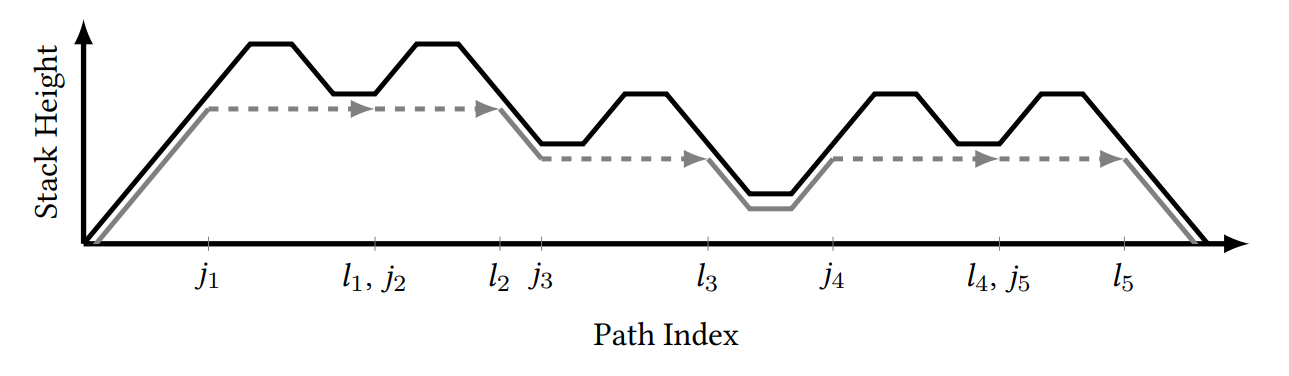
\includegraphics[width=0.75\linewidth]{img/dyck1_path.png}

Сжимаем bell-shaped пути в $\eps$-рёбра. Снова ищем и снова сжимаем. После каждого сжимания мы убираем все локальные максимумы. Чем больше был максимум, тем длиннее $\eps$-ребро. Хуже всего, когда все новые рёбра длины 2. В любом случае путь становится короче хотя бы в 2 раза, так что таких итераций потребуется не более $\log n^2$ (есть лемма, что найдётся путь длины не более $\O(n^2)$). 

\subsubsection{Алгоритм}

Для построения алгоритма воспользуемся следующим результатом:

\begin{lemma}\cite{Deleage1986}

Для языка $L$ определим $p_L(n)$~\footnote{Формально, $p_L(n) = \max \{ \min \{|w| \colon w \in L \cap K \}, K \in Rat_n, L \cap K \ne \varnothing \}$,\\ где $Rat_n(X)$~--- регулярные языки над алфавитом $X$, распознаваемые НКА с $\le n$ состояниями.}~--- максимальная длина кратчайшего слова в $L \cap K$ по всем регулярным языкам $K$, задаваемым НКА с $\le n$ состояниями.

Тогда для языка Дика $D_1$ на одном типе скобок $p_{D_1}(n) = \O(n^2)$
\end{lemma}

\begin{corollary}
    Для любой пары вершин $u, v \in V(G)$, если есть Диков путь $u \path v$, то существует и Диков путь $u \path v$, длина которого $\O(n^2)$.
\end{corollary}
\begin{proof}
    Слова, читаемые на путях $u \path v$ задаются НКА на $n$ вершинах~--- графом $G$, в котором $u$ и $v$ выбраны за начальное и конечное состояния соответственно.
\end{proof}

Пользуясь этим фактом, можно соорудить наивный алгоритм~--- достаточно лишь заметить, что раз длина искомого пути всегда ограничена, то можно задать такие пути с помощью ДКА (язык $D_1$ задаётся автоматом с одним счётчиком, значение счётчика не превышает $\O(n^2)$, так что его можно закодировать в состояние) на $\O(n^2)$ состояниях. 

\TODO: дописать красиво

\textit{Ну тут мотивация простая, если строить автомат по грамматике, то часто он получается экспоненциального размера. Сейчас хотим то же в обратную сторону провернуть. Ещё мотивация: чтобы хранить одну чиселку порядка $n^2$ в считающем автомате нужно всего $\O(\log n)$ бит, так что хочется в такое ограничение и уложиться}\\
\TODO: написать красивые слова



% Опишем КС-грамматику, задающую язык Дика на одном типе скобок, вложенность 

\subsubsection{Время работы}

\TODO: Улучшить обычную оценку (ищем ТЗ отдельно в каждой компоненте РКА)

\begin{note}
Этот результат не обобщается на языки Дика с большим типом скобок. 

Мотивация примерно такая: во1, они сложнее (язык Дика на $\ge 2$ типах скобок~--- такой же мощный как и произвольный КС-язык (теорема Хомского-Шутценбергера, тогда как язык Дика на одном типе скобок вроде как попроще. \textit{Ещё Дик на $\ge 2$ типах скобок генерирует full AFL (Abstract Families of Languages) (что бы это не значило)}), во2, сейчас мы играли на том, что состояние~--- примерно одна чиселка (ну опять-таки, язык Дика на одном типе скобок распознаётся автоматом с одним счётчиком), а для большего типа скобок нужен весь стек.
\end{note}